\documentclass{report}

% need it in .docx form? no problem!
% pandoc -s chapter-1.tex -o chapter-1.docx --bibliography="chapter-1.bib"; mv chapter-1.docx ~/Desktop

\usepackage{import}
\import{../}{gov-style}
\addbibresource{chapter-1.bib}

\begin{document}
\begin{refsegment}

\section{The OPM hack}
In April 2015, a security engineer named Brendan Saulsbury was performing a routine security upgrade for the US Office of Personnel Management (OPM) when he noticed some suspicious network activity. From somewhere within OPM, a computer was sending brief updates to a website registered at opmsecurity.org---a domain address designed to look like an official system, but not actually belonging to the US Government or the OPM security team. Saulsbury alerted Curtis Mejeurm, one of OPM's senior IT strategists, and it quickly became clear that this bit of outbound traffic was the surface marker of an iceberg-scale data breach. The US Computer Emergency Readiness Team set up shop the next day in an adjacent basement room and hunkered down to investigate and destroy the malware. 10 days, 2000 items of malware, and 1 scheduled power outage later, government security engineers declared that to the best of their knowledge the threat had been removed.\footcite{koerner_inside_2016} But the work to identify the scope of the damage had only just begun.

Almost immediately, it was publicly speculated that the attack originated from China and had connections to the Chinese government.\footcite{spetalnick_china_2015} Though public-facing officials refuse to admit it, internal investigators determined that the department had been the victim of an attack perpetrated by an advanced persistent threat (APT), a formally organized and typically state-sponsored group of hackers.\footcite[Attributing a cyberattack is difficult because hackers have endless means to obscure their orgins. In this case, however, the first clue that investigators found was left there on purpose. A particularly effective group of hackers tied to China has made it a calling card of sorts to register sites using the names of members of Marvel's comic book superhero group, The Avengers. In this case, opmsecurity.org was registered under the name "Steve Rogers," better known as Captain America.]{koerner_inside_2016} Preliminary estimates determined that perpetrators had stolen the personally identifying information of up to 4 million current and former federal employees, including fingerprint data. The hackers had been present in the system for at least half a year.

Within the first month after the breach was discovered, it became clear that the scope of the attack was well beyond the initial estimates. The Chinese had obtained access to an OPM database of applications for security clearance, which exposed not just the personal data of the applicants themselves but also the detailed information they had supplied about their family and friends.\footcite{nakashima_hacks_2015} Millions of social security numbers, job applications, and home addresses were now in the hands of a foreign power, including information about personnel at the highest levels of government. As FBI Director James Comey put it, ``If you have my SF 86, you know every place I've lived since I was 18, contact people at those addresses, neighbors at those addresses, all of my family, every place I've traveled outside the United States. Just imagine if you were a foreign intelligence service and you had that data.''\footcite{nakashima_hacks_2015} And now the Chinese intelligence service did.

So what did the full power of the United States Government do in response to this massive affront to its security systems and the privacy of citizens? Absolutely nothing. Not a single publicly announced action was taken by the Obama administration that could be interpreted as a retaliatory measure against the Chinese government for stealing the personally identifying information of 21 million Americans.  In case you think I'm missing something, here is the transcript from a July 3, 2017 press briefing---two years after the OPM hack---in which ABC's Jonathan Karl grills Press Secretary Josh Earnest about the administration's lack of response to the OPM hack in the context of its recently announced sanctions against Russia for the election interference (emphasis mine):\footcite[You can watch the full exchange via video here. It's pretty awkward.]{gill_earnest_2017}

\begin{quote}
KARL: So when the Chinese hacked OPM in 2015 [...] \textbf{why did the White House do nothing publicly in reaction to that hack, which, in some ways, was even more widespread than what we saw here from the Russians}, allegedly?
\newline \newline
EARNEST: Well, I think that what we've seen is that \textbf{these are two cyber incidents that are malicious in nature, but materially different.}
\newline \newline
KARL: Twenty-one million people had their personal data taken.  Fingerprints, social security numbers, background checks -- I mean, this was a far-reaching hack.
\newline \newline
EARNEST: I'm not downplaying the significance of it, \textbf{I'm just saying that it's different than seeking to interfere in the conduct of a U.S. national election.} I can't speak to the steps that have been taken by the United States in response to that Chinese malicious cyber activity.\footcite[Transcript adapted from the official White House website.]{earnest_press_2017}
\end{quote}

But... why? What is it about election interference that demands a material sanction from the US Government that is not true of enormous data theft? Karl doesn't let the Press Secretary off the hook with respect to the severity of the incident, correctly pointing out that the harm to US citizens is comparable. The difference, though Earnest was either not equipped or not interested in saying so, is that in this case the government continuously characterized the OPM attack as a form of traditional espionage---spying to build up a database of information about US officials.\footcite{nakashima_chinese_2015}

That intelligence gathering is its own unique category of cyberattack---meriting a separate set of norms---is not explicitly codified anywhere. Instead, it is one of the generally understood ``rules of the road'' of international espionage. The Congressional Research Service report about the incident quotes an unnamed Senior Administration Official who makes this distinction. According to them, The White House has been clear ``that there is a vast distinction between intelligence-gathering activities that all countries do and the theft of intellectual property for the benefit of businesses in the country, which we don't do and we don't think any country should do.'' The not-at-all subtle implication is that espionage for other purposes \emph{is} something that we do, and don't necessarily think other countries should refrain from doing either. The CRS report concludes that as of now, the OPM breach ``appears to be seen in the category of intelligence-gathering, rather than commercial espionage.''\footcite{finklea_cyber_2015} And though he avoided repeating it, James Clapper, director of national intelligence, went so far as to say ``you have to kind of salute the Chinese for what they did,'' explicitly condoning a certain level of interstate espionage and offering a tacit acknowledgment of why further sanctions were not pursued.\footcite{sanger_u.s._2015}

Back to Earnest, who confirms that, with only 17 days left in power, the Obama administration had completely opted against any public retribution:

\begin{quote}
KARL: But nothing was announced. There was not a single step announced by the White House in response to that.
\newline \newline
EARNEST: That is true that there was no public announcement about our response, but I can't speak to what response may have been initiated in private.
\newline \newline
KARL: \textbf{But no diplomats expelled, no compounds shut down, no sanctions imposed, correct?}
\newline \newline
EARNEST: Well, again, I can't speak to --
\newline \newline
KARL: \textbf{You don't do that stuff secretly.}  I mean, that's --
\newline \newline
EARNEST: Well, certainly when it comes to the diplomats, that's right, there were no diplomats PNGed. That's something that we would announce publicly.
\end{quote}

Not only can you not do ``that stuff'' secretly, establishing norms and deterring future malicious behavior would seem to require that you do it as publicly as possible. The White House even acknowledged that they needed to be more public in their response for the purposes of deterring attacks like the OPM hack.\footcite{sanger_u.s._2016} Supposedly, they considered covert cyber-retaliation measures as well as putative economic sanctions, though the latter of never materialized.\footcite{nakashima_hacks_2015} Obama administration officials refused until the very end to name China as the culprit. A September 2018 press conference with Trump administration National Security Advisor John Bolton was the first time a US Government official formally attributed the OPM hack to the Chinese government.\footcite{sanger_trump_2018} By then the window for a comeback response was long gone.

There are a number of high-profile cyberattacks in recent years to chose from, but the OPM hack best illustrates the central question that motivates this thesis: why does the United States appear to allow a number of highly damaging cyberattacks to happen without meaningful public retribution? The 2018 National Cyber Strategy of the United States of America is undoubtedly correct when it states that ``Russia, Iran, and North Korea conducted reckless cyber attacks that harmed American and international businesses and our allies and partners without paying costs likely to deter future cyber aggression.''\footcite{trump_national_2018} Do we in fact have to accept James Clapper's premise, and salute the Chinese for an honest piece of intelligence work?

I propose that the United States policy response to cyberattacks often feels disproportionately muted because in cases where the attack is deemed to be solely an intelligence operation, the response is informed by the already-established norms of peacetime espionage. These norms form a pattern of behavior between states in which espionage is formally denounced, but punished in the most perfunctory possible manner. In this way the international community maintains an equilibrium where states attempt to frustrate each others' ability to gather intelligence, but do not impose punishments that would discourage the attempt at espionage or cause the punished party to crack down on espionage against them in a similar manner. I will provide evidence that this equilibrium exists in a variety of intelligence contexts, and present possible explanations for why the international community continues to maintain it.

Whether norms influence state behavior or are subordinate to realist power dynamics is a foundational debate in IR scholarship. It is not debatable, however, that the desire to establish and maintain some set of cyber norms is a motivating factor for policymakers at the highest levels of government. The current National Cyber Strategy claims that its goal is to promote ``adherence to voluntary non-binding norms of responsible state behavior that apply during peacetime.''\footcite[p.~20]{trump_national_2018} With regards to the question of cyber espionage's permissibility, ranking House Intelligence Committee member Adam Schiff (D-Calif.) stated with surprising candor that ``We want to draw a bright line” that hacking for economic benefit “is a violation of international norms,'' in contrast to other forms of hacking.\footcite{nakashima_hacks_2015} John Brennan, Director of the CIA, was even willing to say that spying on each others' political institutions is ``fair game.''\footcite{sanger_u.s._2016} In this thesis, I hope to answer why the US seeks to maintain that distinction, and why pretty much every major power in the international systems agrees to treat certain forms of espionage as permissible.

\section{A brief history of US cyber policy}
\subsection{Domestic law and international strategy}
In order to understand how espionage norms influence United States cyberpolicy, it is important to first understand the hole in the legal framework that espionage helps to fill. Absent comprehensive, enforceable treaties, there is no separate set of laws that guide the prosecution of domestic and international cyber crimes.\footnote{There are, of course, \emph{some} treaties that deal with international cyber law. They are however few and far between, and with the possible exception of the Budapest Convention, mostly irrelevant to the decision-making of major actors today. I do not have time to comprehensively address that in this draft the way that I will the domestic law, but I imagine some analysis of the existing norms interplay with the nascent cyber treaties will make its way into this thesis.} There are only the domestic laws, with which we can prosecute domestic criminals or foreign nationals who happen to wander into friendly territory, and whatever ability we have to compel compliance with international norms. As such, an overview of how the United States has evolved in its definition of cyberattack and associated repercussions for perpetrating one is necessary.

Over the second half of the \nth{20} century, policymakers began the process of defining the nature and consequences of what would come to be called a cyberattack. Computer and network security had been a concern for government officials since computers were first integrated into public offices, but it took a long time before cybersecurity in a broader sense would be recognized as the crucial battlefront that it is today. Early policy recommendations for securing government computers focused on addressing specific types of vulnerabilities, rather than broader strategic concerns.

A reasonable place to start in the history of cybersecurity policy is with a General Accounting Office recommendation from 1977 titled ``Security of Computer Systems.''\footcite{washington_post_staff_timeline_2003} Delivering the report in testimony before the Congressional Subcommittee on Consumer Affairs, GAO director Donald Scantlebury warned that Government computer systems were insufficiently prepared to defend against ``actions such as crimes, espionage, mischief, and sabotage.''\footcite{u.s._government_accounting_office_security_1977} In the report, he uses the example of a ``computer burglar'' to illustrate how malicious entities might use computer systems to gain access to confidential information or submit fraudulent requests for payment. After a few attempts, Congress and the Reagan administration passed the first federal computer crime legislation seven years later,\footcite[This later bill, the Computer Security Act of 1987, describes the 1984 bill as being the first federal legislation in this area.]{glickman_computer_1988} the ``Counterfeit Access Device and Computer Fraud and Abuse Act of 1984,'' which made it a federal offense to produce a ``fraudulent access device.''\footcite{hughes_access_1984}

The first recognized computer worm (a type of virus) was unleashed on the early internet by Robert Morris, a Cornell graduate student in 1988, supposedly by accident. The self-replicating virus crashed thousands of computers connected the to government's internet precursor, ARPAnet, before it finally was  contained a few days later.\footcite[This source, a master's thesis for the USAF Air University, makes the dramatic and completely unsubstantiated claim that the Morris worm infected half of of ARPAnet's 88,000 computers. The more popular (and plausible) claim is that of the roughly 60,000 ARPAnet-connected computers, the worm infected 10\% of them, though that number is not particularly well substantiated either.]{moore_conception_2014} A GAO report requested by Congress in the event's aftermath noted that cases like these were still somewhat difficult to prosecute due to the lack of federal statutes directed at computer-virus-type incidents.\footcite{u._s._government_accounting_office_computer_1989} That didn't stop the Justice Department from making an example out of Morris as one of the first felony convictions under the Computer Fraud and Abuse Act. The worm and its aftermath permanently altered the public perception of the internet, which until then had felt ``like a small town where people thought little of leaving their doors unlocked.''\footcite{lee_how_2013}

The relevance of this history to US foreign policy with respect to cybersecurity is twofold. First, it illustrates the continuous development of the legal framework under which the United States government evaluates the harm---and justifies a response---to an abstract domestic cyberattack. The application of domestic laws to international practice is one of the ways in which international legal norms are formed.\footcite[p.~295]{deeks_international_2015}  Even though there is not yet a robust body of law governing cyberspace, documented state practice presents a pattern by which we can begin to establish customary cyber law.\footcite[p.~129]{brown_customary_2012} And prosecuting cyber intrusions domestically at the very least ensures that no state can claim a ignorance to its illegality or argue that cyber intrusions are somehow legally undefined.

Second, the Morris Worm and dearth of available laws with which to respond to it demonstrates the relative recency of the moment in which the inevitability of a malicious attack on federal computer systems was first taken seriously. There simply hasn't been that much time for a comprehensive body of law to form, let alone a body of law that deals with cyberattacks that originate internationally. Robert Morris was a bored 23 year-old who wanted to see how much of the nascent internet his program could reach and unintentionally demonstrated its massive potential for harm. But though his mistake primed policymakers to consider the danger of such an attack, it also set a precedent for thinking of cyberattacks as a one-off. A terrorist or a teen might seek to infiltrate the Department of Defense, and they ought to be prosecuted in response, but there was no external political implication attached. What that external political implication should be is something that policymakers struggle with to this day.

For the remainder of the \nth{20} century, the Federal Government stepped up its focus on securing ``critical infrastructure.'' The George H. W. Bush White House because the first administration to issue a directive treating network security as a pressing national security issue. The official objective of National Security Directive 42 was, perhaps a bit redundantly, ``Ensuring the security of national security systems.'' The government was waking up to the sheer extent to which their critical infrastructure was vulnerable to a cyberattack, but NSD-42 does not actually address the likelihood of, much less the proper method of responding to, an attack originating from a hostile foreign power.\footcite{bush_national_1990}

Between 1992 and 2000, the internet and its potential for commerce and society became abundantly clear to American society. President Clinton firmly integrated cybersecurity into the broader strategic planning of national security and defense, even if it wasn't quite clear at the time what they were protecting and how they planned to do it. In September 1993, Clinton issued Executive Order 12864, which established the Council on the National Information Infrastructure. The definition of a National Information Infrastructure is left rather vague, but it essentially describes the public structure that would come to be known as the World Wide Web: ``hardware, software and skills that will make it easy and affordable to connect people with each other, with computers, and with a vast array of services and information resources.'' In 1996, Executive Order 13010 created the President's Commission on Critical Infrastructure Protection, designed to protect ``critical infrastructures from physical and cyberthreats and assuring their continued operation.'' In this space, ``Critical Infrastructure'' has a more well-defined meaning, understood to cover utilities like water, power, fuel, telecommunications, and financial services.\footcite[~p.761. Completely omitted from this thesis is the concurrent debate about the role the government should play in regulating encryption technology. At the same time it was drafting the Executive Orders mentioned above, the Clinton administration was also taking executive action to manage encryption. The encryption debate (which is still ongoing today) raises a lot of questions about the relationship between the federal government, civil liberties, and law enforcement, as well as more generic national security concerns. It is however mostly irrelevant the specific international political questions that motivate this inquriy, and as such is not included here.]{boys_clinton_2018} The inclusion of cyberthreats alongside physical ones signifies a landmark understanding of the actual threat that the internet posed---not just as a new system of infrastructure to defend, but as a vector by which all legacy infrastructure was soon to be made vulnerable as well.

In the last few years of the millennium the first policy recommendations appear that finally recognize how the internet could be be used as a means of attack by a hostile foreign power. CIA Director John Deutch testified to the Senate in 1996 that ``hackers, criminal groups, and foreign intelligence services consider [information systems] lucrative targets,'' noting that a handful of foreign nations have already instituted ``formal information warfare programs.''\footcite{deutch_worldwide_1996} In 1998, Cybersecurity for the first time merited its own section in the annual National Security Strategy, and the subsequent strategy, released the following year, warned that cyberattacks ``could originate from terrorist or criminal groups as well as hostile states.''\footcite[~p.760-761]{boys_clinton_2018} Policymakers and presidents had finally identified the danger of cyberattacks and their potential as a tool for war, but they still weren't conceiving of cyberspace as a unique domain for international competition, one deserving of its own ``rules of the road.''

Jump ahead to the present day, and a few international incidents later, it is clear that cyberattacks are one of the dominant ways that states compete with each other in the international system. Starting with the Clinton administration's National Plan for Information Systems Protection, each American presidential administration has put out a document detailing their cyber strategy.\footnote{In order: "The National Plan for Information Systems Protection" (Clinton), "National Strategy to Secure Cyberspace" (Bush), "International Strategy for Cyberspace: Prosperity, Security, and Openness in a Networked World" (Obama), "National Cyber Strategy of the United States of America" (Trump). The Trump strategy bizarrely claims that it is the "first fully articulated cyber strategy in 15 years." It does not specify whether they simply ignored the Obama-era strategy document or if they don't consider it to be a "fully articulated cyber strategy" for some reason, but the statement is in either case incorrect.} These plans tend to be long, heavy on agencies and committees, and not particularly interesting. Most importantly, they are all incredibly vague as to how the United States will respond to a cyberattack by a foreign power.

Because our current cyber strategy builds on the work of statutes, directives, and norms from past administrations, proving that our stated cyber strategy is lacking in response mechanisms requires looking briefly at each one. The Bush strategy is heavy on the promoting the private sector's responsibility to voluntarily secure their own networks, but it introduced no new enforcement mechanisms, a factor which it was criticized at the time.\footcite{lemos_bush_2003} President Obama introduced quite a few new official directives on the topic of cybersecurity, but for most of his presidency these generally lacked enforcement mechanisms as well. Assessing Obama's efforts to secure the nation against cyberthreats in 2013, PolitiFact outlined the various features of his cyber strategy and its associated directives, then bluntly noted: ``So that's what has happened. What hasn't happened: a change in law.'' The editors gave his promise to ``develop a comprehensive cybersecurity and response strategy'' a grade of ``In the Works.''\footcite{moorhead_work_2013}

It wasn't until the end of the Obama administration that the United States government fully acknowledged that  cyberattacks would happen and avenues for punishment were required. While early cybersecurity strategies focused heavily on defense and prevention, it had now become clear that cybersecurity policy needed to shift its focus towards strategies for mitigation and response. This was a crucial evolution in understanding cyberattacks as a full-featured weapon of diplomacy and war, and it is one that the Trump administration has since embraced. Just as the military would never say that its "missiles strategy" was to not get hit by missiles, so too was it time to stop saying that our cybersecurity strategy was to secure our nation against cyberattacks.

\subsection{Existing structures for cyber repercussions}
To the extent that we have a comprehensive cyber strategy and set of enforcement mechanisms, it is a patchwork of structures set up towards the end of the Obama administration and modified during the Trump administration. There are two Obama-era actions in particular that directly influence our response to cyberattacks today.
The first is Presidential Policy Directive 41, a plan codifying how the federal government rates the severity of a given cyber incident (Figure \ref{severity-schema}), and sets the architecture and principles that guide its response. The other is Executive Order 13694, which authorizes the Secretary of the Treasury ``to impose sanctions on those individuals and entities that he determines to be responsible for or complicit in malicious cyber-enabled activities that are reasonably likely to result in, or have materially contributed to, a significant threat to the national security, foreign policy, economic health, or financial stability'' of the US.\footcite{daniel_our_2015} The order was also later amended to include election interference. Not only did the Trump administration leave the order in place, they quietly extended it in 2017.\footcite{uchill_white_2017}

\begin{figure}
\centering
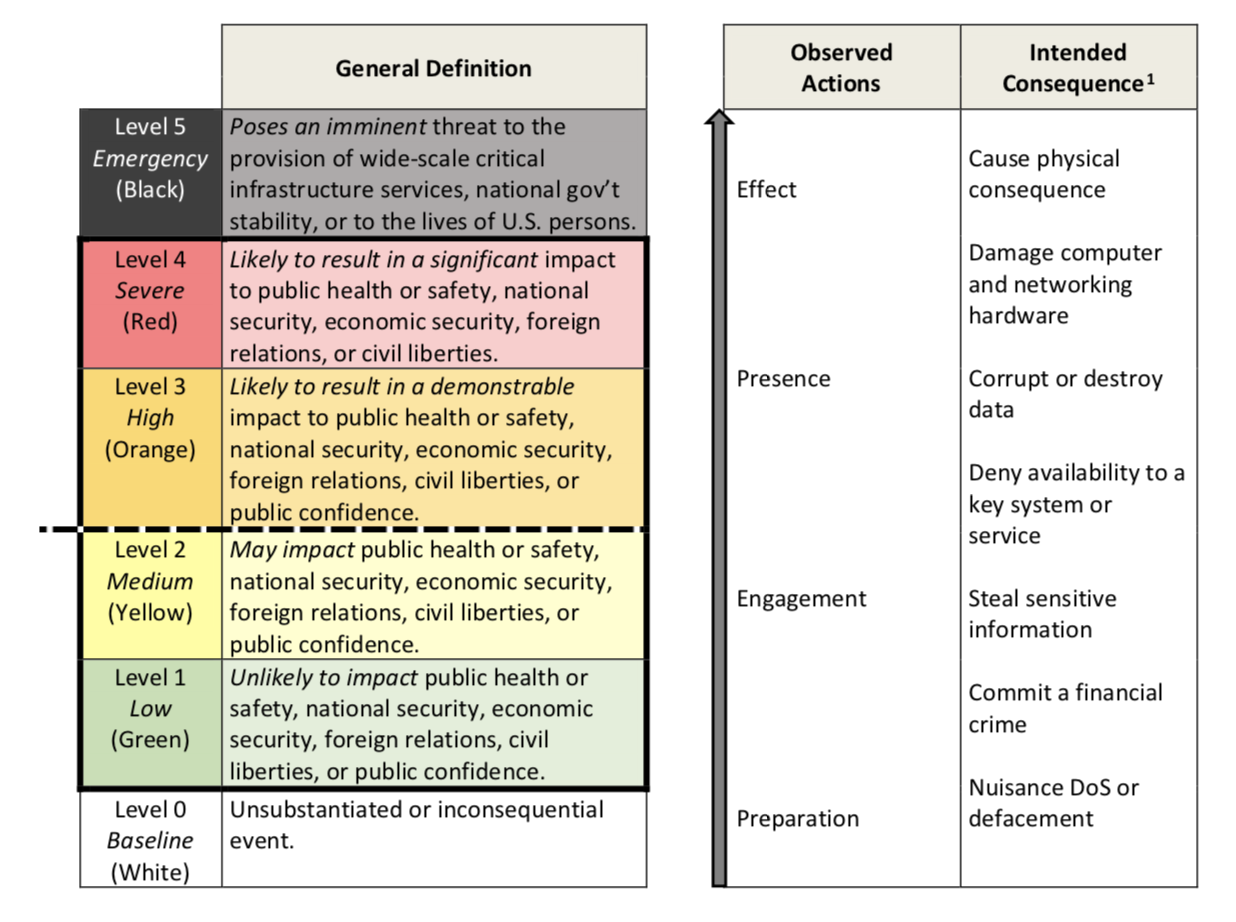
\includegraphics[scale=0.53]{severity-schema.png}
\caption{Cyber Incident Security Schema (The White House 2016)}
\label{severity-schema}
\end{figure}

In fact, despite the controversy surrounding Russian interference in the 2016 election---and President Trump's subsequent reluctance to address or attribute it---so far there really isn't much daylight between his administration's stated strategy on cybersecurity and that of the administration prior. Though more martial and aggressively worded as per his style, Trump's 2018 cybersecurity strategy offers few specifics that contradict any Obama-era strategy. Christopher Painter, former White House Senior Director for Cyber Policy, argues that it ``sends a strong message of continuity to our public and our partners.''\footcite[Painter also served at the State Department for six years as the Coordinator for Cyber Issues, which at the time was an Assistant Secretary level position. Since then, its status within the department has fluctuated wildly. Rex Tillerson, Trump's first Secretary of State, announced that he would abolish the office and merge it into State's Bureau of Economic Affairs. Then, just a few months later, he proposed creating an entirely new department bureau with a Senate-confirmed Assistant Secretary, possibly in response to criticism of his first decision. Though current Secretary Mike Pompeo appears to have more interest in cyber policy, the State Department still has not reestablished a high level cyber position.]{painter_white_2018} Part of the continuity is because a lot of Obama's achievements in the cyber realm were heavily technocratic, and the Trump administration ``National Cyber Strategy of the United States of America'' is light on specifics to contradict them.\footcite{guest_blogger_white_2018} Towards the end of his presidency, Obama signed measures to promote public-private information sharing, secure financial transactions, and establish the Cyber Threat Intelligence Integration Center.\footcite[Among other actions taken during the Obama presidency, these were sufficenct for PolitiFact to update its 2013 rating of his cyber-enforcement actions to ``Promise Kept.'']{carroll_obama_2016} Most of these measures are still on the books, and as far as we know continue to guide our cyber attack response.

The one area in which the Trump administration has pointedly diverged from Obama-era cyber policy is in constraints on the offensive use of cyberattacks, and this particular issue is the locus of questions about what sorts of norms the US operates under (and helps to create) when considering cyber operations. In August 2018, President Trump signed a classified order that rescinded Obama's Presidential Policy Directive 20 and had the practical effect of ``delegating authority to the defense secretary to use cyber tools and techniques to disrupt or degrade an adversary's network or choke off attacks underway''\footcite{nakashima_trump_2018} Previously, such an attack would have to have been vetted by the State Department and intelligence agencies, which some within the DoD and Cyber Command found limiting.

Rescinding PPD-20 is a significant step by the Trump administration to reduce the constraints on US Cyberwarfare operations, though at the risk of shooting from the hip and neglecting other broad concerns (diplomatic, legal, economic) that the military might not weigh equally.\footcite{starks_ramifications_2018} It also reduces some of the incentive to cooperate with civilian intelligence services, increasing the risk that the military might decide to operate without sufficient information, and potentially even compromise an existing operation within a civilian agency.\footcite{hawkins_cybersecurity_2018} General Paul Nakasone, director of both the National Security Agency and the United States Cyber Command, and the person with whom the authority to launch a cyberattack now rests, had expressed frustration during his Senate confirmation hearing that America's adversaries attacked us online with little concern for retaliation.\footcite{sanger_trump_2018}

What is there to learn from this survey of existing enforcement mechanisms? It tell us that when it comes to responding to a cyberattack, the United States government does not lack for options. The Department of the Treasury has the ability to unilaterally impose sanctions on entities suspected of malicious cyber-enabled activities that endanger ``national security,'' a term so broad it might as well be a blank check. The Trump administration made it appreciably easier for the military to engage in offensive cyberattacks, which should theoretically be a deterrent. And of course policymakers still have access to other, more traditional deterrent tools. In response to a damaging cyberattack, the US could expel diplomats from the offending nation, impose financial sanctions on some relevant portion of their economy, or refuse to cooperate on other diplomatic issues until certain conditions are met. Theoretically, they always have the option to launch a missile.

\subsection{Espionage: the missing piece}
As it stands the United States Federal Government, its intelligence agencies, and its military have significant leeway to penalize states and state-sponsored entities for malicious cyber-activities---and it appears that they often choose not to. Presidential administrations have spent 20 years issuing documents that stress the need to increasing our cyber defenses, and the past 5 years issuing documents that promise the United States will respond appropriately to a cyberattack that is ``likely to result in demonstrable harm to the national security interests, foreign relations, or economy of the United States or to the public confidence, civil liberties, or public health and safety of the American people.''\footcite{office_of_the_press_secretary_fact_2016} So when exactly do they choose to use the tools that they have available?

One common excuse you hear from spokespeople is that attributing cyberattacks is difficult, so their retaliatory options are limited by uncertainty. Yes, definitively attributing cyberattacks is difficult, but there is also no external standard of proof that intelligence agencies have to meet in order to justify a response---the relevant policymakers just have to be convinced that the intelligence justifies their actions. That's how we ended up in Iraq. In the case of the OPM hack, investigators were sure from almost the very beginning that the parties responsible were affiliated with the Chinese government. Once the government has determined the origin and the nature of the harm with a sufficient level of certainty, it then falls on the policymakers to determine a response, and that is where the guidelines that the US government publishes cease to have any explanatory power.

How, for instance, does the color-coded severity chart correspond with the relative severity of retaliatory options, like counterespionage or economic sanctions? Does a Level 2 violation (Medium, Yellow) merit a diplomatic protest, but a Level 3 (High, Orange) result in financial sanction? Remember the kinds of espionage that John Brennan said were ``fair game.'' How could a severity ranking possibly mesh with the United States' supposed interest in tacitly permitting cyber operations that look like more classical forms of espionage? The federal government is naturally vague about how it weighs its ``assessment of the risks posed to an entity, national security interests, foreign relations, or economy of the United States or to the public confidence, civil liberties, or public health and safety of the American people,'' but that vagueness renders the response framework toothless to the point of absurdity.\footcite{office_of_the_press_secretary_fact_2016}

These ambiguities are more than theoretical. The OPM hack, for instance, would fall under a Level 2 severity---stealing sensitive information---but under those guidelines, so would Chinese theft of American trade secrets, otherwise known as ``economic espionage.'' Unlike other forms of espionage, the United States does not appear to engage in economic espionage, and takes an active role in promoting norms that discourage it. In 2015, talks between the United States and China resulted in a pact where Chinese President Xi Jinping, ``apparently rattled by the threat of sanctions,'' agreed to affirm a norm against economic espionage.\footcite{nakashima_u.s._2015} That same agreement conspicuously did not include any language curtailing traditional espionage, even though the Chinese had recently perpetrated the attack that compromised the personnel files of the very people doing the negotiating.\footcite{nakashima_u.s._2015} While there will be a more thorough discussion of economic espionage in the last chapter, I mention it now to illustrate two key points: that the stated cyber policy of the United States leaves important ambiguities that can only be resolved by understanding espionage norms, and that if the United States did desire to impose deterrent costs on traditional espionage, it has the tools to do so.

Even in situations where the cyber-severity schema does help us understand some aspects of of our cyber retaliation, it is still incomplete. Compare the government response to the OPM hack with the fallout from the Sony hack of 2014. In the latter, hackers affiliated with the North Korean government stole sensitive information and leaked damaging emails from Sony executives, supposedly in retaliation for the upcoming James Franco/Seth Rogen comedy about assassinating North Korean leader Kim Jong-Un.\footcite{barnes_sony_2017} The government responded swiftly; the Sony hack was first time a sitting US president came out and publicly accused a foreign nation of launching a cyberattack while promising retaliation.\footcite{sanger_u.s._2016} The US actually made good on its threat, and direct sanctions came to North Korea the following year.\footcite{lederman_us_2015} A Washington Post article called the response ``unprecedented.''\footcite{nakashima_why_2015}

One important difference between the two breaches is that in the case of the Sony hack, the North Koreans caused physical damage to the company's servers, corrupting data and destroying hardware, not unlike how Stuxnet caused Iranian centrifuges to spin at uncontrollable, permanently damaging speeds. According to former Obama Administration official Jake Sullivan, that physical element set the Sony hack apart from other cyber-security incidents, and guided the government's stronger response.\footcite[Jake Sullivan served as the Deputy Assistant to the President and National Security Advisor to the Vice President. Piror to that, he was the Director of Policy Planning at the State Department.]{sullivan_personal_2019} This statement is consistent with the severity schema, in which ``Damage computer and networking hardware'' is a Level 4 (Severe, Red) offense, that is ``Likely to result in a significant impact to public health or safety, national security, foreign relations, or civil liberties.'' The Sony Pictures hack would seem to fit within that definition, but it doesn't tell the full story.

Public statements by government officials complicate that straightforward explanation. One factor almost entirely unaccounted for by our cyber policy is the difference between an operation carried out against the US government, and one with the goal of intimidating a private company. The Cyber Security Severity Index doesn't make that distinction clear---but President Obama did. ``We cannot have a society in which some dictators someplace can start imposing censorship here in the United States.''\footcite{perez_obama_2014} Again, administration officials formally acknowledged the crucial role that norms play in guiding international behavior in the cyber realm. ``These lawless acts of intimidation demonstrate North Korea's flagrant disregard for international norms,'' said Secretary of State John Kerry.\footcite{perez_obama_2014} The State Department coordinator for cyber issues even admitted that had Sony not canceled the movie in response---turning the incident into an issue of free speech and American civic values---that it was ``fair to say'' the response might have been more muted, physical damage notwithstanding.\footcite{nakashima_why_2015}

There is probably a way to read the cyber strategy documents outlined in this section such that the public responses the Chinese OPM hack, the North Korean Sony hack, and Chinese economic espionage are internally consistent with stated US strategy. But were such a reading even possible, it would have to be a retroactive justification; there would be no way to come up with the resulting federal response just by looking at American cyber policy.\footnote{The ambiguity I'm discussing here is not unique to cyber policy. There are obviously quite a few areas of American foreign policy where our actions do not line up with our stated principles and policies. The challenge for IR scholars is to tease out which factors nation-states consider when making their decisions. For cyber policy, I am proposing that espionage norms are one of those factors.} The missing variable in this equation is the emerging norms about cybersecurity---the train tracks that the US government is laying down in front of them while simultaneously riding the locomotive.\footnote{See: Wallace and Gromit train tracks gif.} Those cybersecurity norms clearly regard some forms of malicious cyber activity as permissible, and statements by public officials indicate that existing norms of espionage play a key role in how they make that determination.

Are the norms under which we operate a series of conscious decisions in line with the best security, deterrence, and intelligence practices---or are they an outdated port of Cold War espionage norms that see a distinction between types of security breaches were none exists? If we want to use the norms of traditional espionage to understand how the United States federal government evaluates the harm of various cyber attacks, then we need to know what constitutes ``intelligence-gathering activities that all countries do,'' and what norms guide their acceptability. By determining what the international community does or does not consider acceptable in the context of espionage, we can shed light on what the United States intelligence community would consider acceptable in the world of cyber espionage.

President Obama often referred to taming the ``Wild West'' of cybersecurity, by which he meant that absent treaties and international laws, we have only a brief history of norms to guide us, and each decision that we make in response to a cyber incident carries outsized significance in redefining them.\footcite{sanger_u.s._2016} For the purpose of defining norms, the ambiguity of existing cyber policy is a feature, not a bug. It allows American policymakers vast flexibility in determining what forms of cyber activity ought to be formally denounced on the world stage, and which ones are routine espionage they'd rather handle quietly. So in order to understand how those distinctions will be drawn in the future, it is necessary to understand how they formed in the first place, and what purpose they serve.

\section{The norms of espionage}
\subsection{Definition}
So far I have been a bit vague about what ``espionage norms'' actually means. It should be clear by now that certain types of cyber attack resemble traditional forms of espionage, and that policymakers sometimes consider them to by guided by the same norms. But what norms exactly? Is there a particular norm among them that prescribes the appropriate response to an act of espionage?

Norms, by definition, do not impose hard constraints on a state's ability to act---they suggest the contours of what a state will consider appropriate. To understand the norms of a particular field is to understand the range of options on the table and the likelihood that any given one will be chosen. Ideally, those norms are robust enough that it is possible to extrapolate a sort of policy rubric, in this case explaining how one state assesses an intelligence threat and then makes a response. If we understand the criteria by which the threat is evaluated, then we can explain why the government appears to consider only a limited range of responses to major cyberattacks, and predict which types of attack might elicit something stronger.

I propose that a single crucial practice underpins the post-Cold War international consensus on peacetime intelligence gathering: espionage is not explicitly permitted between states, but as long as certain boundaries are not crossed, the state is essentially guaranteed that retaliation will be limited to espionage-curtailing activities in the event that they are discovered. Even after having a particularly damaging intelligence operation uncovered---an agent deep within the adversary's government, for instance---the worst that is likely to happen is the expulsion of foreign nationals working the in embassy under diplomatic cover. Because the embassy personnel expelled are typically those that have been identified as possible intelligence agents, the move to expel diplomats is explicitly aimed at making espionage more difficult in the future; it does not punish the offending state for having attempted the espionage in the first place.

Losing embassy staffers who were identified---likely correctly---as intelligence agents is a legitimate consequence. It guts the embassy's operational presence, which can have a lasting impact on that state's intelligence gathering ability in that nation for years to come.\footcite{macintyre_spy_2018} As far as discouraging espionage goes, however, diplomatic expulsions have all the deterrent effect of a parking ticket. When an embassy staffer is outed as a spy by the host nation, that staffer is still subject to the customary protection of diplomatic immunity. The worst that can happen to them is to be declared \emph{persona non-grata} along with a handful of their colleagues and expelled from the country for ``activities incompatible with their diplomatic status.'' If the spy is not a diplomat, they will be tried and held captive (or killed), and if they are lucky they might get traded. Typically no further penalties are applied to the state that sent them. There will not be economic sanctions, nor linkage that substantively impacts other diplomatic issues, only a variation in the number of diplomats expelled depending on how serious the breach. Like with a parking ticket, you simply pay the fine when you get caught and you're free to drive again.

Occasionally, a state will overstep the customary bounds, and in those cases the consequences are extended just enough to make it clear that this particular action is not within ``the rules the game.'' This still happens today, most recently with the Russian poisoning of retired spy Sergei Skripal, who had been previously traded.\footcite{masters_has_2018} Actions that overstep the boundaries also often take the form of covert operations, such as funding dissidents, enabling a coup, or disseminating propaganda. Though these actions sometimes performed by civilian intelligence agencies---the CIA infamously engineered the overthrow of democratically-elected Guatemalan President Jacobo Arbenez in 1954---the norms governing skullduggery are sufficiently different from the norms governing espionage that they treated by both academic literature and diplomatic practice as entirely different categories of offense.\footcite{fraser_architecture_2005} In many cases, however, these actions are tolerated to a surprising degree as well.
% Add some stuff about deterrence theory here - requested book from the other library

\subsection{Research design}
In the following three chapters, I will examine some of the most significant diplomatic incidents that resulted from intelligence-gathering operations, and assess the international fallout from each. With each case, I will demonstrate that despite ample provocation, the offended party's response was muted and explicitly limited to espionage-related diplomatic actions. In doing so, I make the case that if these incidents which received significant press did not merit a stronger response---or at least one that broadened the scope of the repercussions---then it is virtually impossible that harsh sanctions resulted from some lesser offense that escaped the attention of the public. To be even more specific: if a great power state is caught spying on another in a way that both parties want to be permissible, the absolute worst that will happen in terms of material consequences is tit-for-tat diplomatic expulsions.

Of course, it is possible, even likely, that there are consequences to espionage exposure that are not made public. But it would be difficult to imagine that any such secret consequences have could have a significant deterrent effect.  The most severe repercussions are ones that are felt by the most people, which in turn puts pressure on the offending party and makes it less likely that their leaders are will choose to repeat the undesirable behavior. This is what Jonathan Karl is getting at when he asks Josh Earnst about why there were ``no diplomats expelled, no compounds shut down, no sanctions imposed,'' because ``you don't do that stuff secretly.''\footcite{earnest_press_2017} The norm-breaking consequences, ones which would prove that states impose penalties for attempted espionage that are more significant than diplomatic expulsions, almost by definition have to be public.

The cases that I use to examine this premise are limited to Great Powers in the post-WWII era, for a few reasons. The first is simply scope. The purpose of these cases is to demonstrate that even in the worst instances, the only actions taken in response were limited to espionage-related retaliation. To broaden the time period would make it more difficult to argue that the cases chosen represent that maximal possibilities for diplomatic incident that arise from espionage. And since the Cold War is the historical period that immediately precedes our current one, it can't really be said that these examples are out of date. I also use a pretty loose definition of Great Powers, at the very least including the United States, The Soviet Union, The United Kingdom, and France during the Cold War, adding China and Russia later on. While it is possible that some smaller intelligence services reacted to an incident in a norm-breaking way, they generally deferred to their NATO/Warsaw block superpower when it came time to respond. If an incident did not rise to the level of their concern, than it probably has no norm-defining power in this context.

Present-day espionage institutions also have significant operational holdover from the Cold War, having been founded either shortly before (Britain's MI6, 1909), during (United States' CIA, 1947), or immediately after (Russia's FSB, 1995). Many of the intelligence techniques used today were developed in an environment where two superpowers were actively seeking new methods to undermine each other that, by design, fell short of conventional war. Espionage is one such method. The Truman doctrine is another. Though that geopolitical environment no longer exists, the norms that it spawned absolutely do.

The other reason that I focus on the Cold War is because peacetime espionage as we understand it today, performed continuously by civilian intelligence agencies, did not really exist before the Second World War. As I will further explain in Chapter 3, President Truman was initially skeptical that a civilian intelligence agency was even necessary after the war ended. Prior to 1945, countries certainly ran spies and covertly messed with affairs of their rivals, but to nowhere the extent that emerged during the Cold War, when it became one of if not the dominant mode by which states compete in the international arena.

How does one establish what the ``most significant'' intelligence-related incidents of the Cold War were? Crudely, they're the ones you've probably heard of. Julius and Ethel Rosenberg. Gary Powers in the downed U-2 spy plane. The Iran-Contra affair. The controversies which reached the press are the ones that would have applied the most pressure to leaders to respond in kind. In the interest of applying some scholarly rigor, however, I have broken espionage into three categories that compose the same number of chapters: aerial reconnaissance, human intelligence, and satellites. With the first two, there is a rich history of diplomatic incidents which I can analyze for evidence of norms. For the latter, the complete absence of anti-satellite conflict is a noteworthy example of the norm which I hope to prove.

Those three categories cannot hope to cover the rich field of intelligence. I explicitly exclude covert operations, which attempt to sabotage or influence, while intelligence operations attempts to inform. The Iran-Contra affair is not an espionage incident that falls within my definition. I do, however, believe that they provide a wide enough scope to cover the most serious diplomatic incidents that resulted in the field of intelligence, and sufficiently demonstrate how even the most damaging espionage is handled in such a way to continue preserving its practice.


% Let's define an ``espionage incident'' as one which in which it was exposed that a person of import was working as an active agent of a foreign government, and that the intelligence they provided was used to inform the foreign government's actions. The presence of a human agent isn't strictly necessary, but in practice the reveal of a successful SIGINT (signals intelligence) or TECHINT (technical intelligence) operation almost never registers beyond the confines of intelligence agencies.\footnote{The exception that proves the rule here is when the Snowden leaks revealed in 2013 that the NSA was tapping German Chancellor Angela Merkel's phone. A counterfactual is impossible, but it's noteworthy that the incident was made public by a third party instead of the German intelligence agency. Rather than provoke incident, the typical reaction to discovering a SIGINT operation is simply to counteract it.} Actively abetting a foreign government by providing them government secrets is about the most serious an allegation possible that still remains entirely within the world of espionage. In the United States, this would land the perpetrator upwards of 20 years in prison. In the USSR they would likely end up dead.


\section{Literature review}
\subsection{Examining norms without espionage}
There is an existing base of literature that attempts to define, or even construct, the norms of cybersecurity out of whole cloth. This approach has its strengths, in particular that it draws upon the existing theoretical literature about international relations norms. Constructivist literature about IR norms is robust and contains important insights about how norms develop in unprecedented situations like the sudden emergence of information warfare. Later on, this thesis will define norms along the lines of this literature base, focusing in particular on ``regulative norms that prescribe, proscribe, and order'' state behavior,\footcite{bjorkdahl_norms_2002} often also called ``the rules of the road.''

The problem with this literature base is that is also tends to be rather generic. It is certainly helpful to understand how states like the US are putting pressure on the international system to implement stricter norms to cyberspace, in the absence of a strong legal framework.\footcite[~p.7]{finnemore_constructing_2016} Likewise noting the lack of strong enforcement mechanisms as a barrier to the formation of norms today helps explain why leaders describe cybersecurity as ``The Wild West''.\footcite{iasiello_what_2016} But while these theoretical underpinnings help bolster the argument that these norms both can regulate state behavior and that states are actively trying to create them, but that doesn't help determine exactly what the norms themselves are.

There are also those who point to existing cases of cyberattacks, analyzed the state's response, and hypothesize that they constitute norms. This is a solid approach, but it works best when the hypothesis is based in a norm that existed prior to the introduction of the internet as a vector for its use. Otherwise, you simply don't have enough cases for it to have any normative force, and the argument is either mostly theoretical\footcite{neutze_cyber_2013} or too specific to be of general use.\footcite{caso_rules_2014} A few articles have actually looked at a particular cybersecurity practice in the context of evolving espionage norms,\footcite{libicki_coming_2017} and attempted to define the ones that they see as emerging, such as the norm against using espionage for private economic gain.\footcite{rascoff_norm_2016} These are the closest to my actual research design---though they don't set out to create a comprehensive framework for state behavior.

\subsection{Espionage through the law}
We can also use older analyses of the role of espionage in interstate competition to shed some light on how cyber espionage is viewed today. As Congressman Schiff put it: ``traditional foreign intelligence activities [...] may look untraditional now that they’re in the cyber realm,'' but they essentially follow the same set of rules.\footcite{nakashima_hacks_2015} Many of the papers that discuss norms in the espionage world actually do so using the legal system as an entry point, even though espionage itself exists in an international legal gray area.\footcite{beim_enforcing_2018} That gray area is precisely why a constructivist analysis of interstate norms is not just useful, but necessary.

While international law does address the topic of intelligence gathering during wartime, it is completely silent on the concept of peacetime espionage.\footcite{radsan_unresolved_2007} Instead, norms around peacetime espionage have typically been analyzed in the context of domestic law.\footcite{demarest_espionage_1995} This is curious, because there are obvious diplomatic considerations that affect how we handle foreign nationals convicted of espionage, yet no international acknowledgment of the practice exists, so informal norms must fill the gap.

And naturally there are those who have attempted to jump straight analyzing the potential for cyberlaw to resolve existing issues. A number of these papers are prescriptive, which this paper fundamentally is not, and they attempt to provide a framework for cyber operations either in a civilian\footcite{yurcik_internet_2001} or military\footcite{kehler_rules_2017} legal context. Some even attempt to place existing norms, like the norm against economic espionage, into the context of international law.\footcite{lotrionte_countering_2015} None, however, have simply set out to define what is or is not permissible in a cyber espionage context, laws or otherwise, and that is what this thesis hopes to do.



% \section{Research design}
% This thesis seeks to establish the feasibility of evaluating United States cyberattack response through the lens of existing espionage norms. That requires that the thesis be split up into two main sections. The first section will establish what norms were developed by intelligence agencies during the Cold War that might be relevant to cybersecurity today. In it, I will look through examples of Cold War espionage incidents and determine how their risk and response were evaluated by the relevant agencies. While this research will be conducted with an eye towards the way these norms might be in active use today, the argument in this part will simply focus on establishing which norms existed that might be relevant to cyberspace at all.

% The Cold War is a richly studied period of American history with clear relevance to today, and at the time of this writing I've just cracked the surface. So far, I've found a some denser anthology\footcite{andrew_secret_2009} books\footcite{johnson_intelligence_2015} that purport to be comprehensive readers on topics in US intelligence. While working on those, I will also be scouring intelligence\footcite{prados_william_2009} histories\footcite{prados_presidents_1996} as well. Armed with a little context on the more obvious intelligence norms we see today, I think I can spot patterns in what sorts of missions and operations were deemed acceptable in the past. There is also the possibility that I come across a more comprehensive compilation of espionage norms, in which case this section of the paper can be dramatically shorter, as it no longer bears the burden to prove these norms by itself.

% There is another interesting contemporary source for espionage norms as well. Whenever a spy operation breaks into the mainstream news, publications often seek out subject matter experts to comment on whether the operation as it played out public view is something that fits within existing intelligence norms. This raises two possibilities for my research. The first is simply noting these contemporary spy incidents that have nothing to do with cyber, and if they indicate the presence of a norm. A relevant example that comes up up in both cyber and traditional contexts is the expelling (or PNGing) of diplomats who are known to be agents of foreign intelligence services.\footcite{risen_rules_2001} Though considered a ``rare and provocative action,'' it's one that Obama took in the wake of the 2016 election hacking scandal, in direct continuity with existing practices for responding to especially provocative forms of espionage.\footcite{mazzetti_game_2017} The second possibility is that I could interview a few of these subject matter experts, either in the academic or military realm. Plans for this do not yet exist, but if it happens, it has significant potential benefits. Much of the history of intelligence is inherently oral, and the best way to figure out the rules of the game is to ask someone who knows how to play.

\newpage
\printbibliography[heading=subbibliography]

\end{refsegment}
\end{document}
